%
% $RCSfile: diagrams.tex,v $
%
% Copyright (c) 2002-2007. Christian Heller. All rights reserved.
%
% Permission is granted to copy, distribute and/or modify this document
% under the terms of the GNU Free Documentation License, Version 1.1 or
% any later version published by the Free Software Foundation; with no
% Invariant Sections, with no Front-Cover Texts and with no Back-Cover
% Texts. A copy of the license is included in the section entitled
% "GNU Free Documentation License".
%
% http://www.cybop.net
% - Cybernetics Oriented Programming -
%
% Version: $Revision: 1.2 $ $Date: 2007-08-01 13:59:00 $ $Author: christian $
% Authors: Christian Heller <christian.heller@tuxtax.de>
%

\chapter{Diagrams}
\label{diagrams_heading}
\index{Diagrams}
\index{Unified Modeling Language}
\index{UML}
\index{Template Diagram}
\index{TD}
\index{Model Diagram}
\index{MD}
\index{Organisation Diagram}
\index{OD}
\index{Communication Diagram}
\index{CD}

Because of the different programming philosophy behind CYBOP, standard
\emph{Unified Modeling Language} (UML) diagrams cannot be used unalteredly for
the design of CYBOL applications. Some of them, however, could be quite useful,
when adapted a bit. For creating CYBOL applications, the following four can be
considered sufficient. They model the structure of:

\begin{enumerate}
    \item \emph{Template Diagram} (TD): one design-time template (hierarchical,
        ontological concept), with purely unidirectional relations; does not
        illustrate relations between different concepts, as these are only
        established by logic models at runtime; could look like a UML class
        diagram (CsD) or a tree, only that a template may not only represent states,
        but also logic (algorithms, workflows) (figure \ref{template_diagram_figure})
    \item \emph{Model Diagram} (MD): the runtime model tree; comparable to UML
        object diagram, but a simple tree with named nodes would suffice; is
        important because input/ output parameters of operations are given as
        dot-separated paths to runtime knowledge tree models (figure \ref{model_diagram_figure})
    \item \emph{Organisation Diagram} (OD): template directories; could look
        like a UML component- or package diagram or a simple tree (figure \ref{organisation_diagram_figure})
    \item \emph{Communication Diagram} (CD): a network of communicating
        systems, which may run on the same or on different physical machines
        (nodes); could look like a UML distribution diagram; not to be mixed
        up with UML collaboration diagram (figure \ref{communication_diagram_figure})
\end{enumerate}

\begin{figure}[ht]
    \begin{center}
        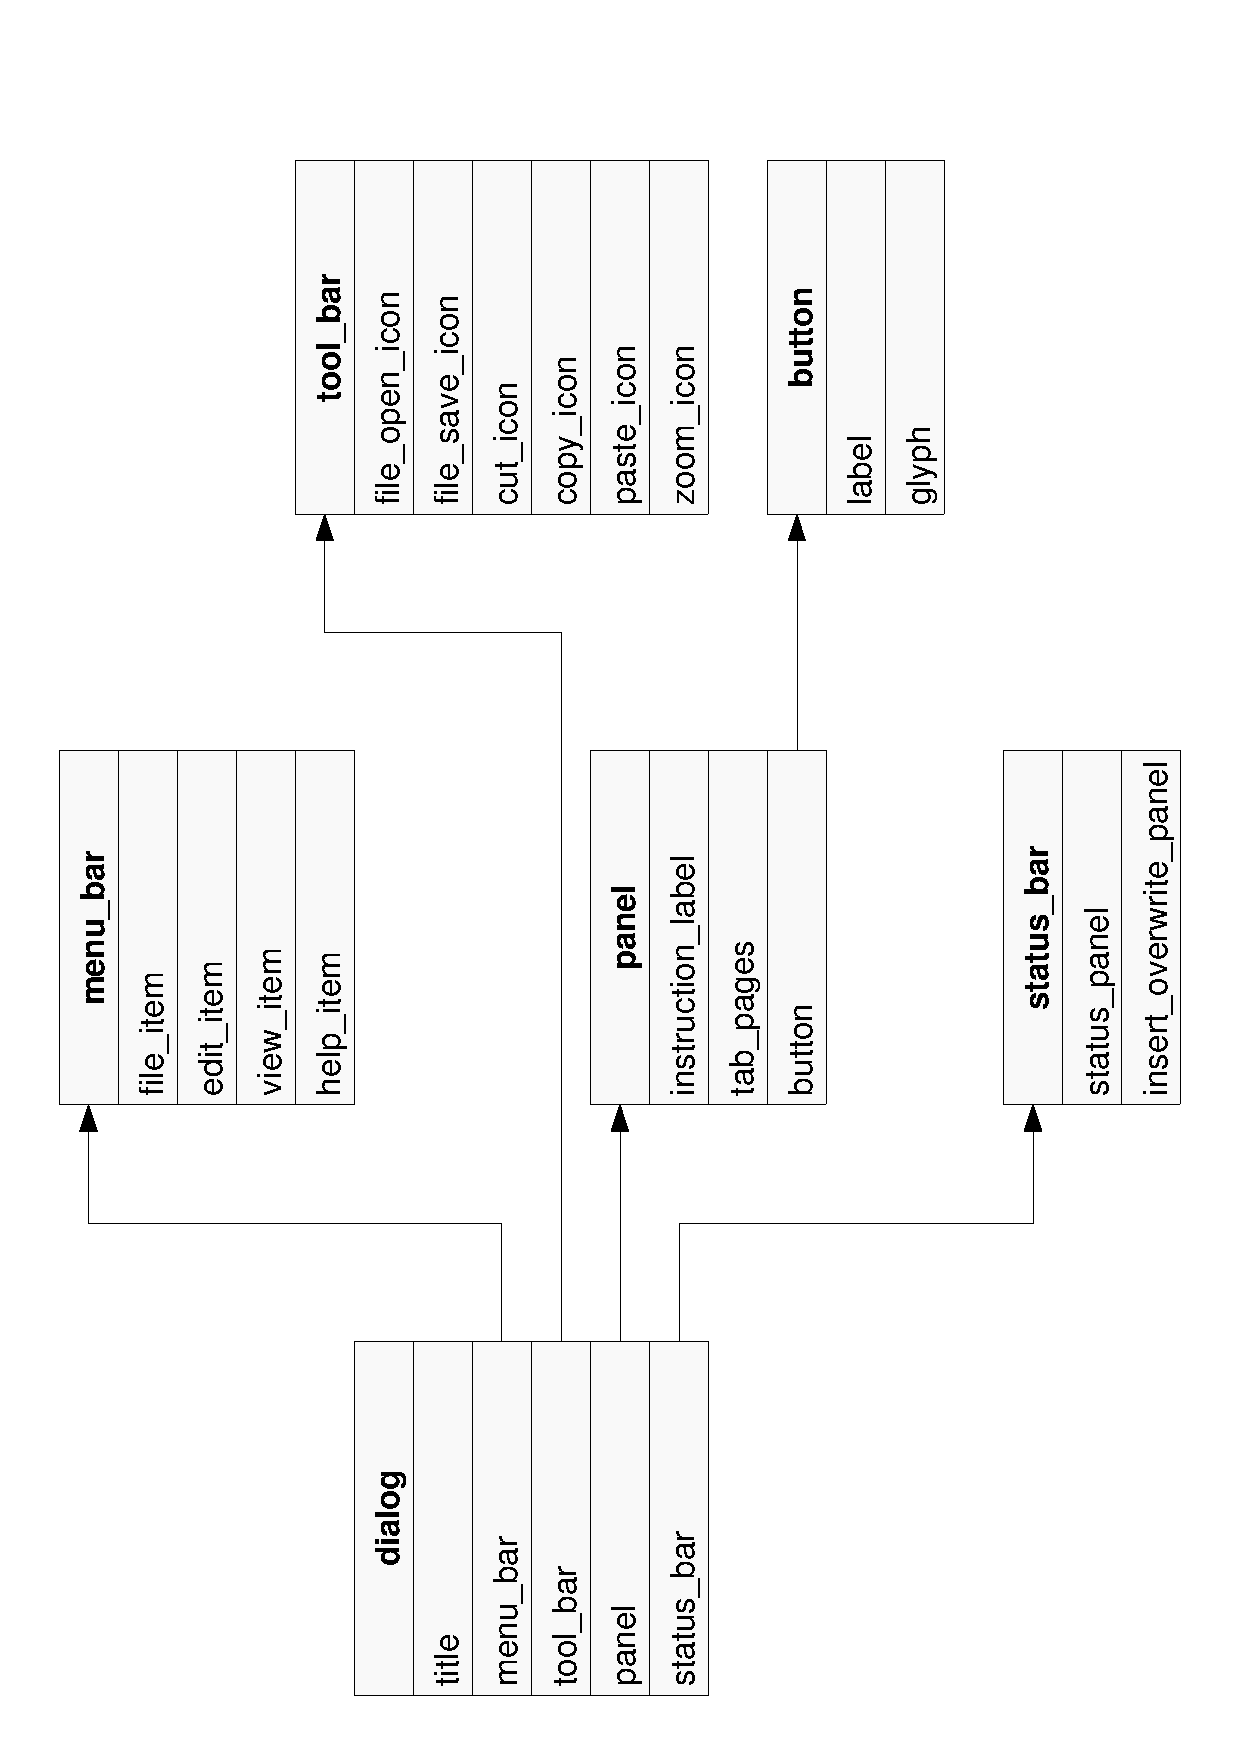
\includegraphics[scale=0.3,angle=-90]{graphics/template_diagram.pdf}
        \caption{CYBOL Template Diagram (TD) Proposal}
        \label{template_diagram_figure}
    \end{center}
\end{figure}

\begin{figure}[ht]
    \begin{center}
        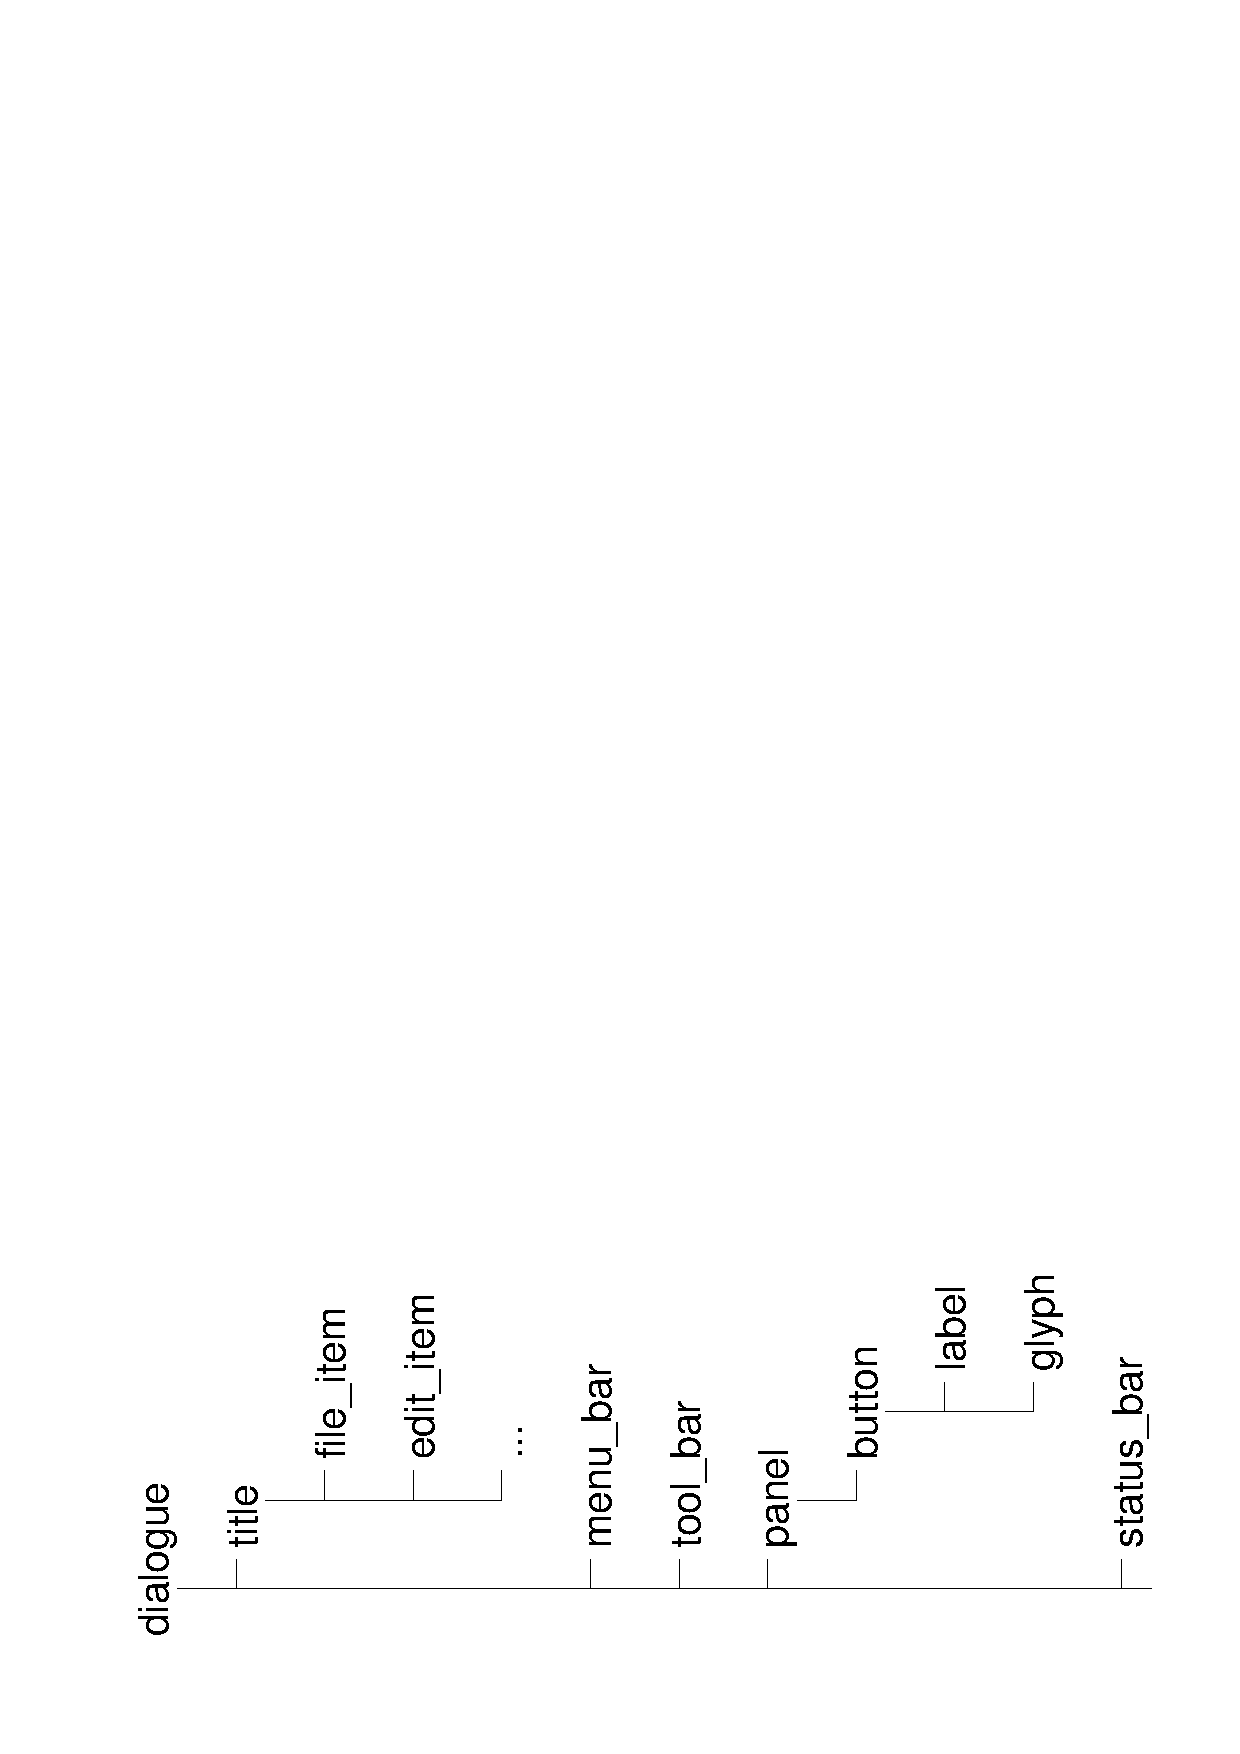
\includegraphics[scale=0.3,angle=-90]{graphics/model_diagram.pdf}
        \caption{CYBOL Model Diagram (MD) Proposal}
        \label{model_diagram_figure}
    \end{center}
\end{figure}

\clearpage

As said above, the four diagrams may look similar to their corresponding UML
pendant. One possible proposal is given for each diagram type. The TD in figure
\ref{template_diagram_figure} illustrates a graphical dialogue. The diagram
looks pretty similar to a UML CsD. Attributes and methods are not bundled in
one concept though, and inheritance does not exist. Associations are drawn if a
concept links to an external concept which may reside in another file (like the
\emph{menu\_bar}), for example. If a part (like the \emph{title}) is hold
inline in the concept, on the other hand, an association is not displayed. Upon
clicking on a part in a concept box, a dialogue opens up that allows the entry
of meta data like the part's channel, abstraction, model and further properties
(details).

The MD in figure \ref{model_diagram_figure} displays the runtime models that were
instantiated with knowledge templates providing the initial values. Again, the
parts of a graphical dialogue were used.

\begin{figure}[ht]
    \begin{center}
        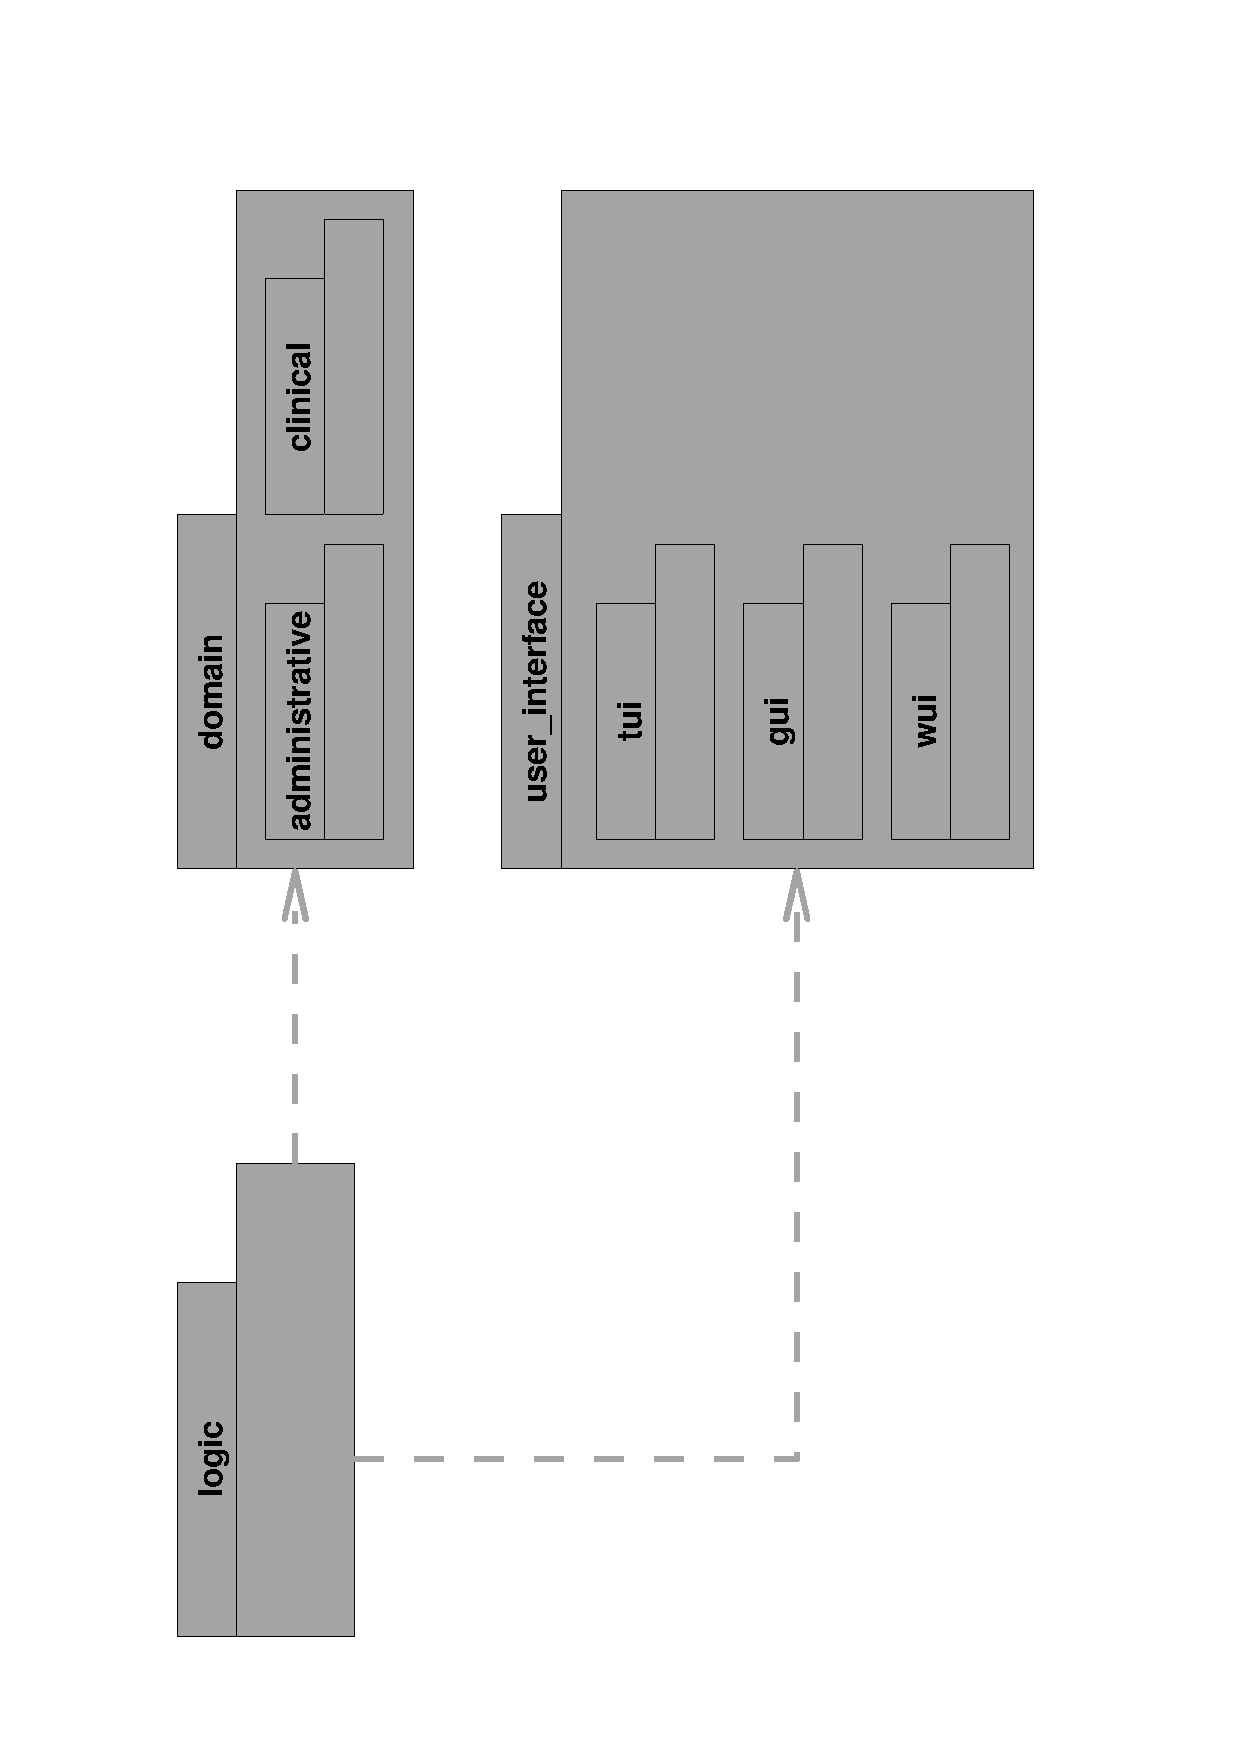
\includegraphics[scale=0.3,angle=-90]{graphics/organisation_diagram.pdf}
        \caption{CYBOL Organisation Diagram (OD) Proposal}
        \label{organisation_diagram_figure}
    \end{center}
\end{figure}

The OD in figure \ref{organisation_diagram_figure} shows packages into which CYBOL knowledge
templates may be organised. Packages do normally correspond to directories on
file system level. The figure contains a \emph{domain} package consisting of
two sub packages, one containing knowledge templates for \emph{administrative}
patient data and the other holding templates for \emph{clinical} data of a
patient. Also, there is a \emph{User Interface} (UI) package containing three
sub packages, for: \emph{Textual UI} (TUI), \emph{Graphical UI} (GUI) and
\emph{Web UI} (WUI). Both, \emph{domain-} as well as \emph{user\_interface}
packages may be accessed from the operations residing in the \emph{logic}
package.

\begin{figure}[ht]
    \begin{center}
        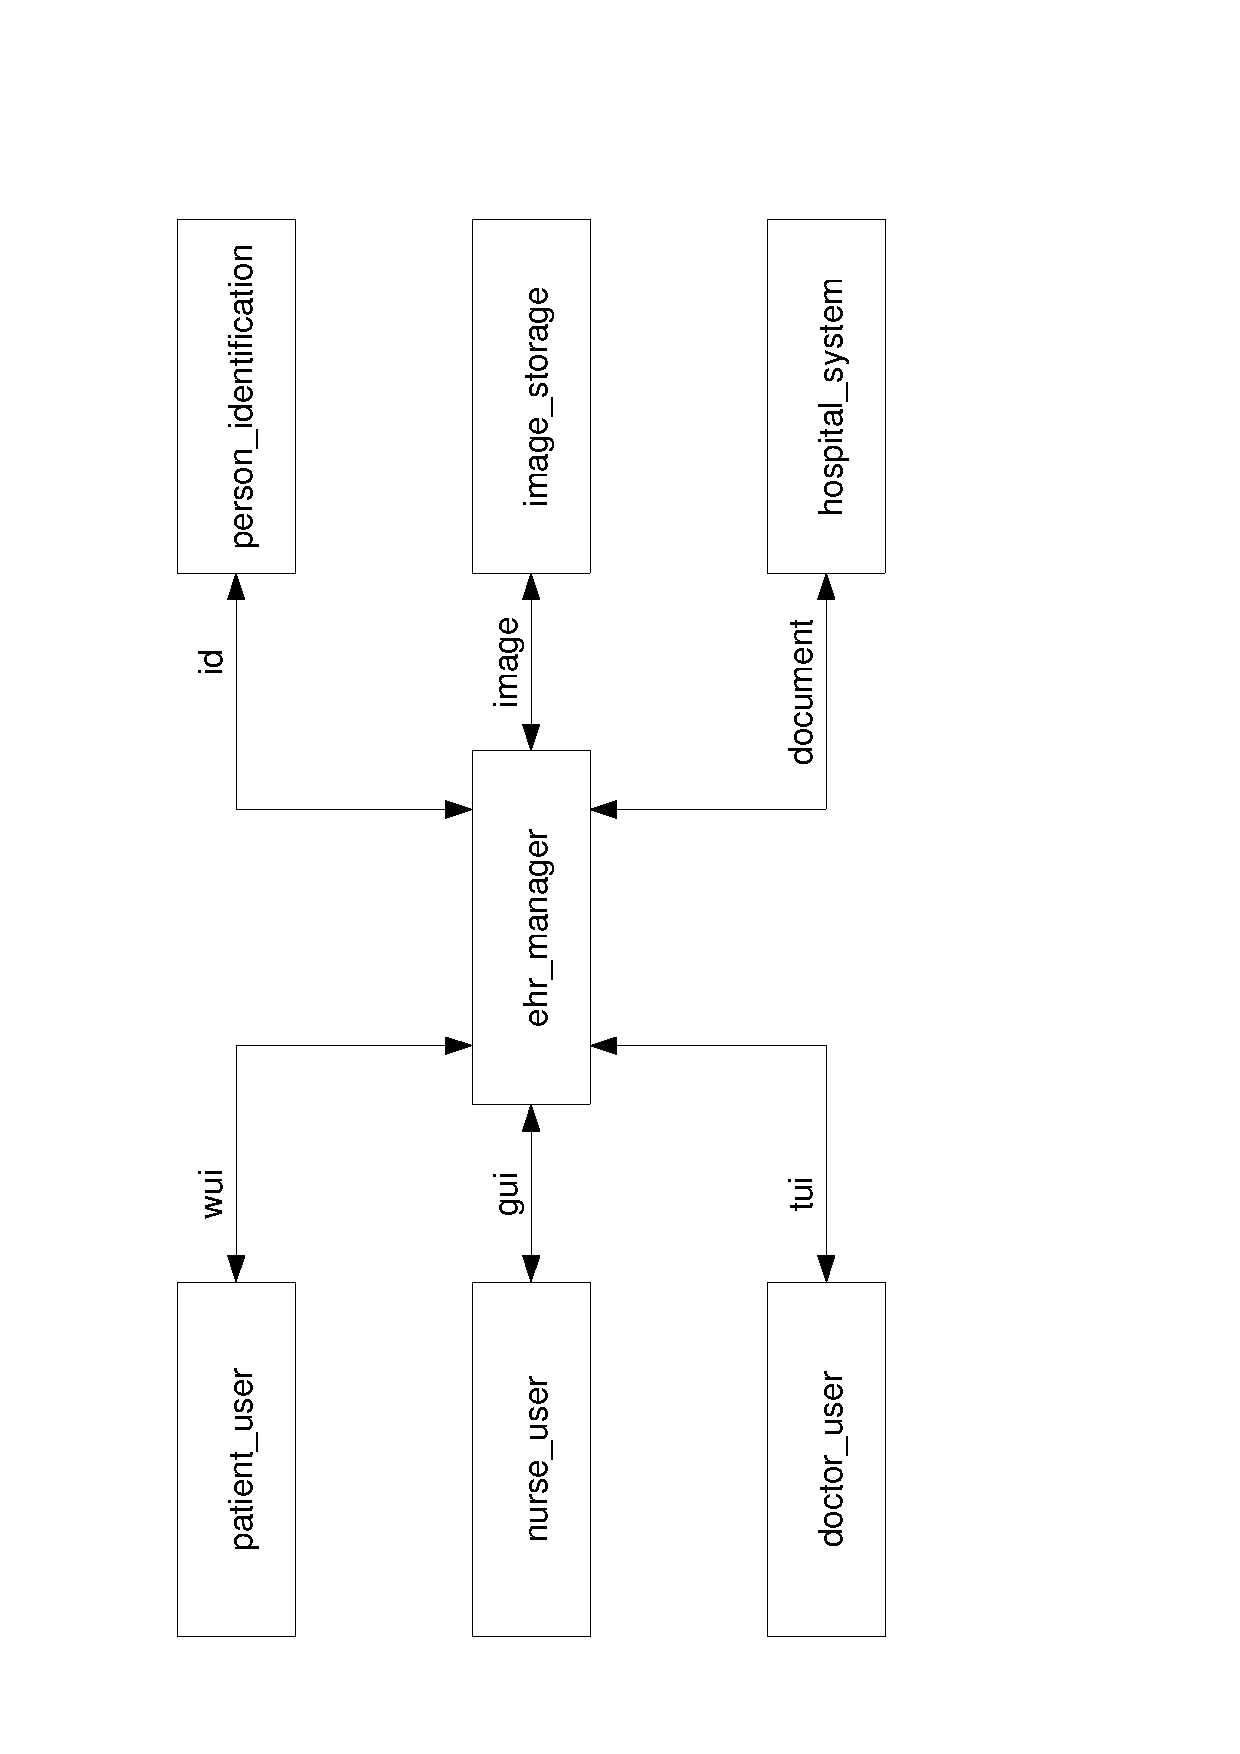
\includegraphics[scale=0.3,angle=-90]{graphics/communication_diagram.pdf}
        \caption{CYBOL Communication Diagram (CD) Proposal}
        \label{communication_diagram_figure}
    \end{center}
\end{figure}

The CD in figure \ref{communication_diagram_figure}, finally, shows a number of independent systems
communicating with each other. An \emph{Electronic Health Record} (EHR) manager
application may be found in the center of the figure. Patients communicate with
it using a WUI; nurses using a GUI and doctors using a TUI (for better
performance). A patient gets identified by asking a \emph{person\_identification}
service. Documents may be exchanged with a \emph{hospital\_system} and images
with a special \emph{image\_storage} system.
